\chapter{R\'ealisation du syst\`eme}
\label{chap:realisation}

\section{Introduction}

Ce chapitre pr\'esente l'environnement reproductible, l'organisation du code et
les interfaces essentielles du prototype. Il d\'ecrit uniquement les composants
pr\'esents dans le d\'ep\^ot et distingue le mode local du mode de d\'emonstration
conteneuris\'e.

\section{Environnement de d\'eveloppement}

\subsection{Environnement mat\'eriel}

Le d\'ep\^ot ne fixe pas un mod\`ele de poste ni une quantit\'e de m\'emoire comme
pr\'econdition. Les caract\'eristiques d'une machine de d\'eveloppement ne sont donc
pas invent\'ees ici. La reproductibilit\'e repose sur les fichiers de verrouillage,
les images Docker à somme de contr\^ole et les contr\^oles pr\'ealables qui
enregistrent les r\'esultats propres à l'h\^ote d'ex\'ecution.

\subsection{Environnement logiciel}

L'environnement de travail associe Arch Linux, Neovim et les outils du projet.
Pacman gère les paquets système, tandis que \texttt{uv} et \texttt{npm}
isolent les dépendances applicatives. Le tableau distingue ces outils de
production du code des composants nécessaires à l'exécution du prototype.

\begingroup
\small
\renewcommand{\arraystretch}{1.16}
\rowcolors{3}{EmeraldWash}{white}
\begin{longtable}{@{}>{\bfseries\color{PremiumEmerald}}p{0.17\textwidth}>{\raggedright\arraybackslash}p{0.32\textwidth}>{\raggedright\arraybackslash}p{0.44\textwidth}@{}}
  \caption{Environnement logiciel et rôle des principaux outils}\label{tab:software-environment}\\
  \rowcolor{PremiumEmerald}\color{white}\bfseries Usage & \color{white}\bfseries Outils & \color{white}\bfseries Rôle \\
  \endfirsthead
  \rowcolor{PremiumEmerald}\color{white}\bfseries Usage & \color{white}\bfseries Outils & \color{white}\bfseries Rôle \\
  \endhead
  Poste & Linux, Arch Linux, pacman & Environnement de développement et installation des paquets système. \\
  Édition & Neovim (nvim), terminal, Zsh, Bash & Écriture du code, exécution des commandes et scripts d'automatisation. \\
  Automatisation & Make, Git, GitHub Actions & Commandes communes, historique des modifications et validation continue. \\
  Dépendances & Python 3.12, uv, Node.js, npm & Environnements Python et JavaScript, dépendances et fichiers de verrouillage. \\
  Calcul et ML & NumPy, pandas, SciPy, scikit-learn, joblib, SHAP & Préparation des données, entraînement, sérialisation et explication des modèles. \\
  Analyse & Jupyter, Matplotlib, nbconvert & Exploration, graphiques scientifiques et export des carnets en HTML. \\
  API & FastAPI, Pydantic, Uvicorn & Validation des entrées et service des routes HTTP et WebSocket. \\
  Données & SQLAlchemy, Alembic, SQLite, PostgreSQL 17 & Accès aux données, migrations, transactions et file persistante. \\
  Interface & TypeScript, React 19, Vite & Composants, typage, serveur de développement et compilation de l'interface. \\
  Visualisation & D3, ECharts, Cytoscape, Lucide & Graphiques, topologie d'investigation et icônes. \\
  Tests & pytest, Vitest, Storybook, Playwright, Axe, Ruff & Tests Python, composants, parcours navigateur, accessibilité et analyse statique. \\
  Déploiement & Docker Engine, BuildKit, Docker Compose, NGINX & Construction des images, orchestration locale et passerelle web. \\
  Réseau & Suricata, Mosquitto, NFStream & Signatures sur paquets, trafic MQTT du laboratoire et extraction PCAP hors ligne. \\
  Sécurité et suivi & Argon2id/pwdlib, PyJWT, OpenSSL, client Prometheus & Hachage, jetons, génération des secrets et exposition des métriques. \\
  Rapport & LaTeX, latexmk, Mermaid CLI, librsvg & Composition du document et rendu vectoriel des diagrammes. \\
  \bottomrule
\end{longtable}
\rowcolors{2}{}{}
\endgroup

\section{Organisation de la r\'ealisation}

\begin{description}
  \item[Machine learning.] Le paquet \texttt{iot\_ids\_ml} s\'epare sch\'ema,
  pr\'eparation, entra\^inement, \'evaluation, promotion et validation des
  artefacts. Le manifeste de production lie mod\`eles, m\'etadonn\'ees et rapport
  par sommes de contr\^ole.

  \item[Backend.] L'application FastAPI s\'epare routes, validation des
  caract\'eristiques, registre de mod\`eles, inf\'erence, ingestion, surveillance
  et persistance. Le traitement durable associe une bo\^ite de r\'eception, des
  transitions immuables et une outbox transactionnelle.

  \item[Frontend.] L'application React est organis\'ee par espaces fonctionnels:
  supervision, alertes, mod\`eles, laboratoire d'observations et topologie. Les
  adaptateurs de \texttt{api.ts} conservent la s\'eparation entre contrats r\'eseau
  et composants visuels.
\end{description}

\section{Principaux choix d'impl\'ementation}

\subsection{Du modèle entraîné à la prédiction servie}

La cascade ex\'ecute toujours le d\'etecteur binaire. Le classifieur de famille
n'est appel\'e que si le premier \'etage retourne une attaque; cette d\'ependance
est conserv\'ee dans les versions et les mesures retourn\'ees. Le registre refuse
un artefact dont le sch\'ema, l'ordre des variables ou les sommes de contr\^ole ne
correspondent pas au manifeste actif.

Le même ordre de 83 variables est contrôlé à l'entraînement et à l'inférence.
Le rejeu permet d'exercer cette chaîne avec les données enregistrées sans
réentraîner le modèle. Les explications SHAP sont calculées à la demande pour
l'investigation ; elles décrivent les contributions au résultat du modèle.

\subsection{Ingestion durable et traitement des erreurs}

L'ingestion HTTP valide un lot complet avant toute insertion. L'identifiant
d'\'ev\'enement et l'empreinte du contenu assurent l'idempotence. Le travailleur
r\'eserve ensuite un travail, ex\'ecute la cascade et valide dans une transaction
l'observation, la pr\'ediction, l'alerte \'eventuelle, la transition et les
messages d'outbox. La diffusion temps r\'eel ne commence qu'apr\`es cette
validation.

Une nouvelle soumission identique n'ajoute pas une seconde observation ; un
contenu différent sous le même identifiant est refusé. Après une erreur
temporaire, le travail est repris avec un délai et un nombre d'essais bornés.
Les échecs persistants sont isolés pour permettre leur examen et une relance
manuelle authentifiée, avec conservation du motif.

\subsection{Interface, contrôle d'accès et provenance}

L'interface conserve trois port\'ees distinctes: les agr\'egats persist\'es du
tableau de bord, la page d'alertes charg\'ee et les \'ev\'enements re\c{c}us pendant
la session. Cette distinction \'evite de pr\'esenter une activit\'e locale du
navigateur comme une mesure historique globale.

La session opérateur utilise un jeton à durée limitée ; l'interface traite
son expiration et les refus de l'API. L'identité associée à une qualification
provient du jeton validé, et non d'un nom libre fourni par le navigateur.
Les vues présentent les états de chargement, d'erreur et de reconnexion pour
éviter qu'une donnée ancienne soit confondue avec un état actualisé.

Dans le laboratoire, Suricata observe le trafic MQTT et HTTP du réseau Docker
isolé. L'agent transmet les événements avec une identité machine distincte.
L'interface affiche leur origine de signature ; ils ne traversent pas la cascade
RT-IoT2022. NFStream reste une voie d'extraction PCAP hors ligne distincte.

\subsection{Exécution reproductible}

\texttt{make setup} prépare les dépendances ; \texttt{make verify-model}
contrôle le bundle promu. Le mode \texttt{make demo} prépare un rejeu initial
dans une base temporaire. Le laboratoire complet démarre avec
\texttt{make demo-sensor}. Ces modes alternatifs facilitent une démonstration
maîtrisée. Les migrations sont appliquées avant le démarrage des services,
et les sondes de santé permettent de vérifier leur disponibilité.

\clearpage
\section{Principales interfaces graphiques}

\subsection{Supervision op\'erationnelle}

La figure~\ref{fig:implementation-monitoring} regroupe l'\'etat de la cha\^ine de
service, la progression du rejeu et les indicateurs d'ingestion. Les valeurs
sont associ\'ees à leur port\'ee afin de distinguer historique persist\'e et
activit\'e de la session.

\begin{figure}[htbp]
  \centering
  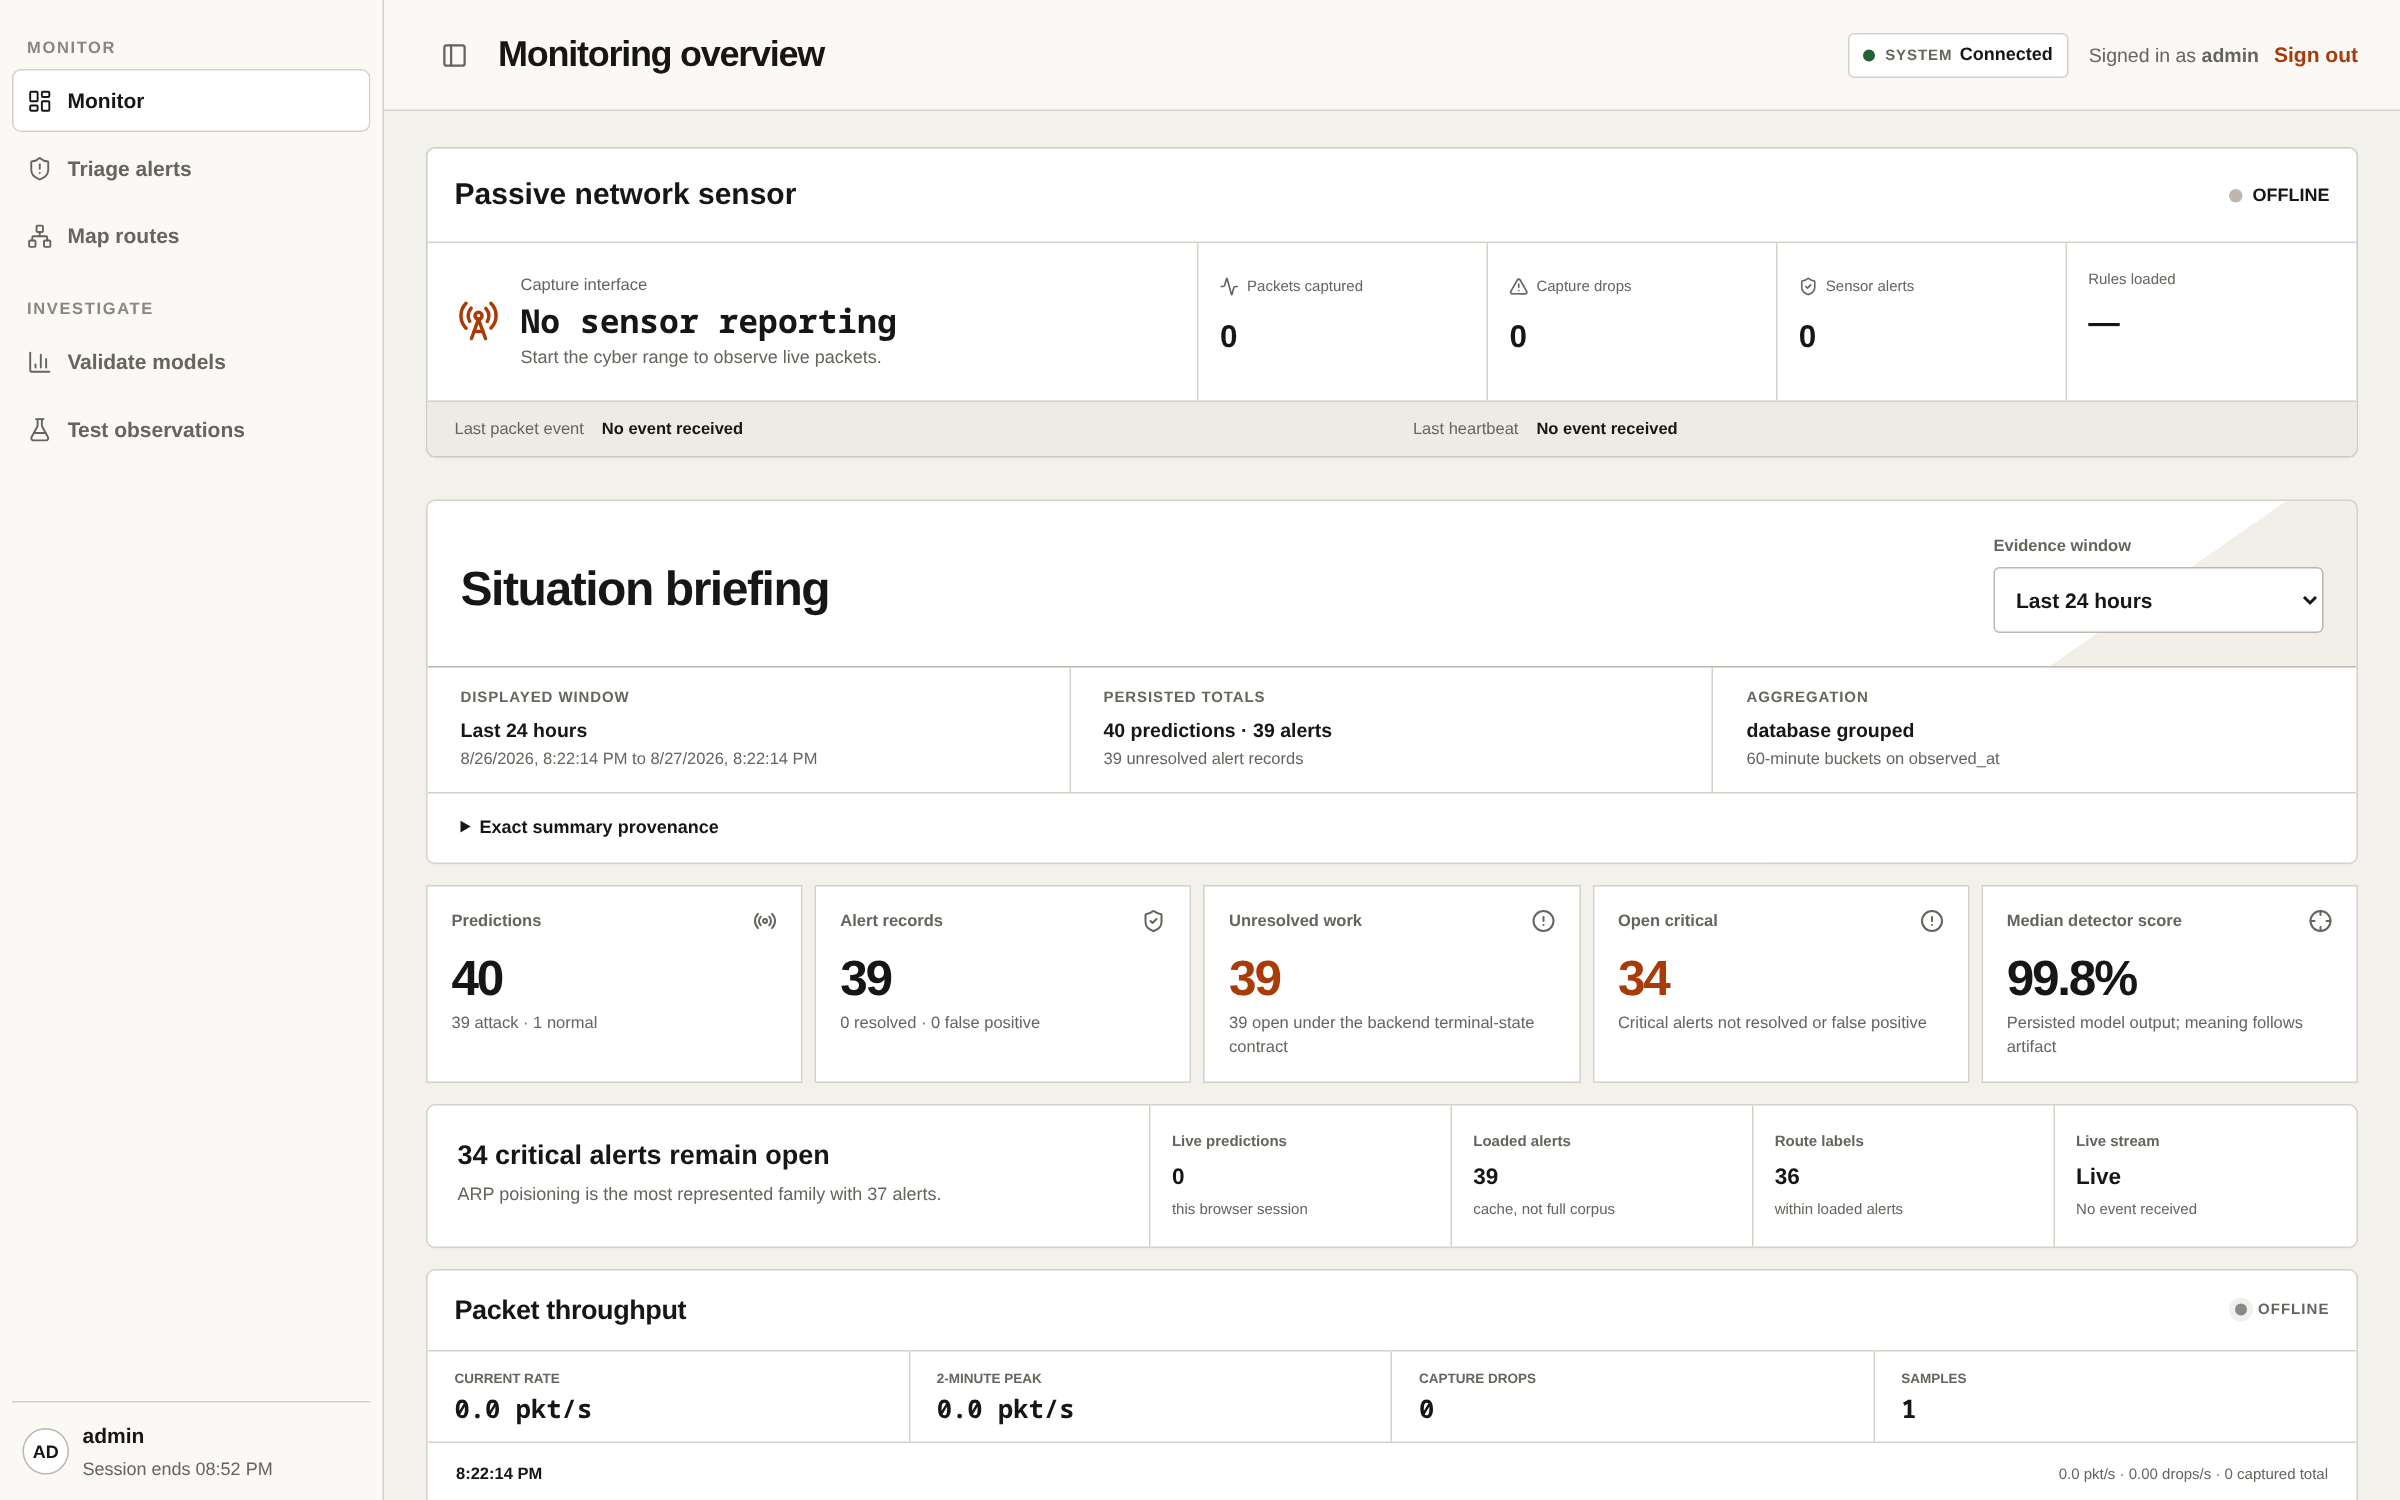
\includegraphics[width=\textwidth,height=0.65\textheight,keepaspectratio]{assets/screenshots/application-monitoring.png}
  \caption{Espace principal de supervision du prototype}
  \label{fig:implementation-monitoring}
\end{figure}

\clearpage
\subsection{Investigation des alertes}

La figure~\ref{fig:implementation-alerts} pr\'esente la file filtrable et le
point d'entr\'ee de l'investigation. Le d\'etail distingue l'origine ML de
l'origine Suricata et conserve la provenance, les scores, les versions et
l'historique de qualification disponibles.

\begin{figure}[htbp]
  \centering
  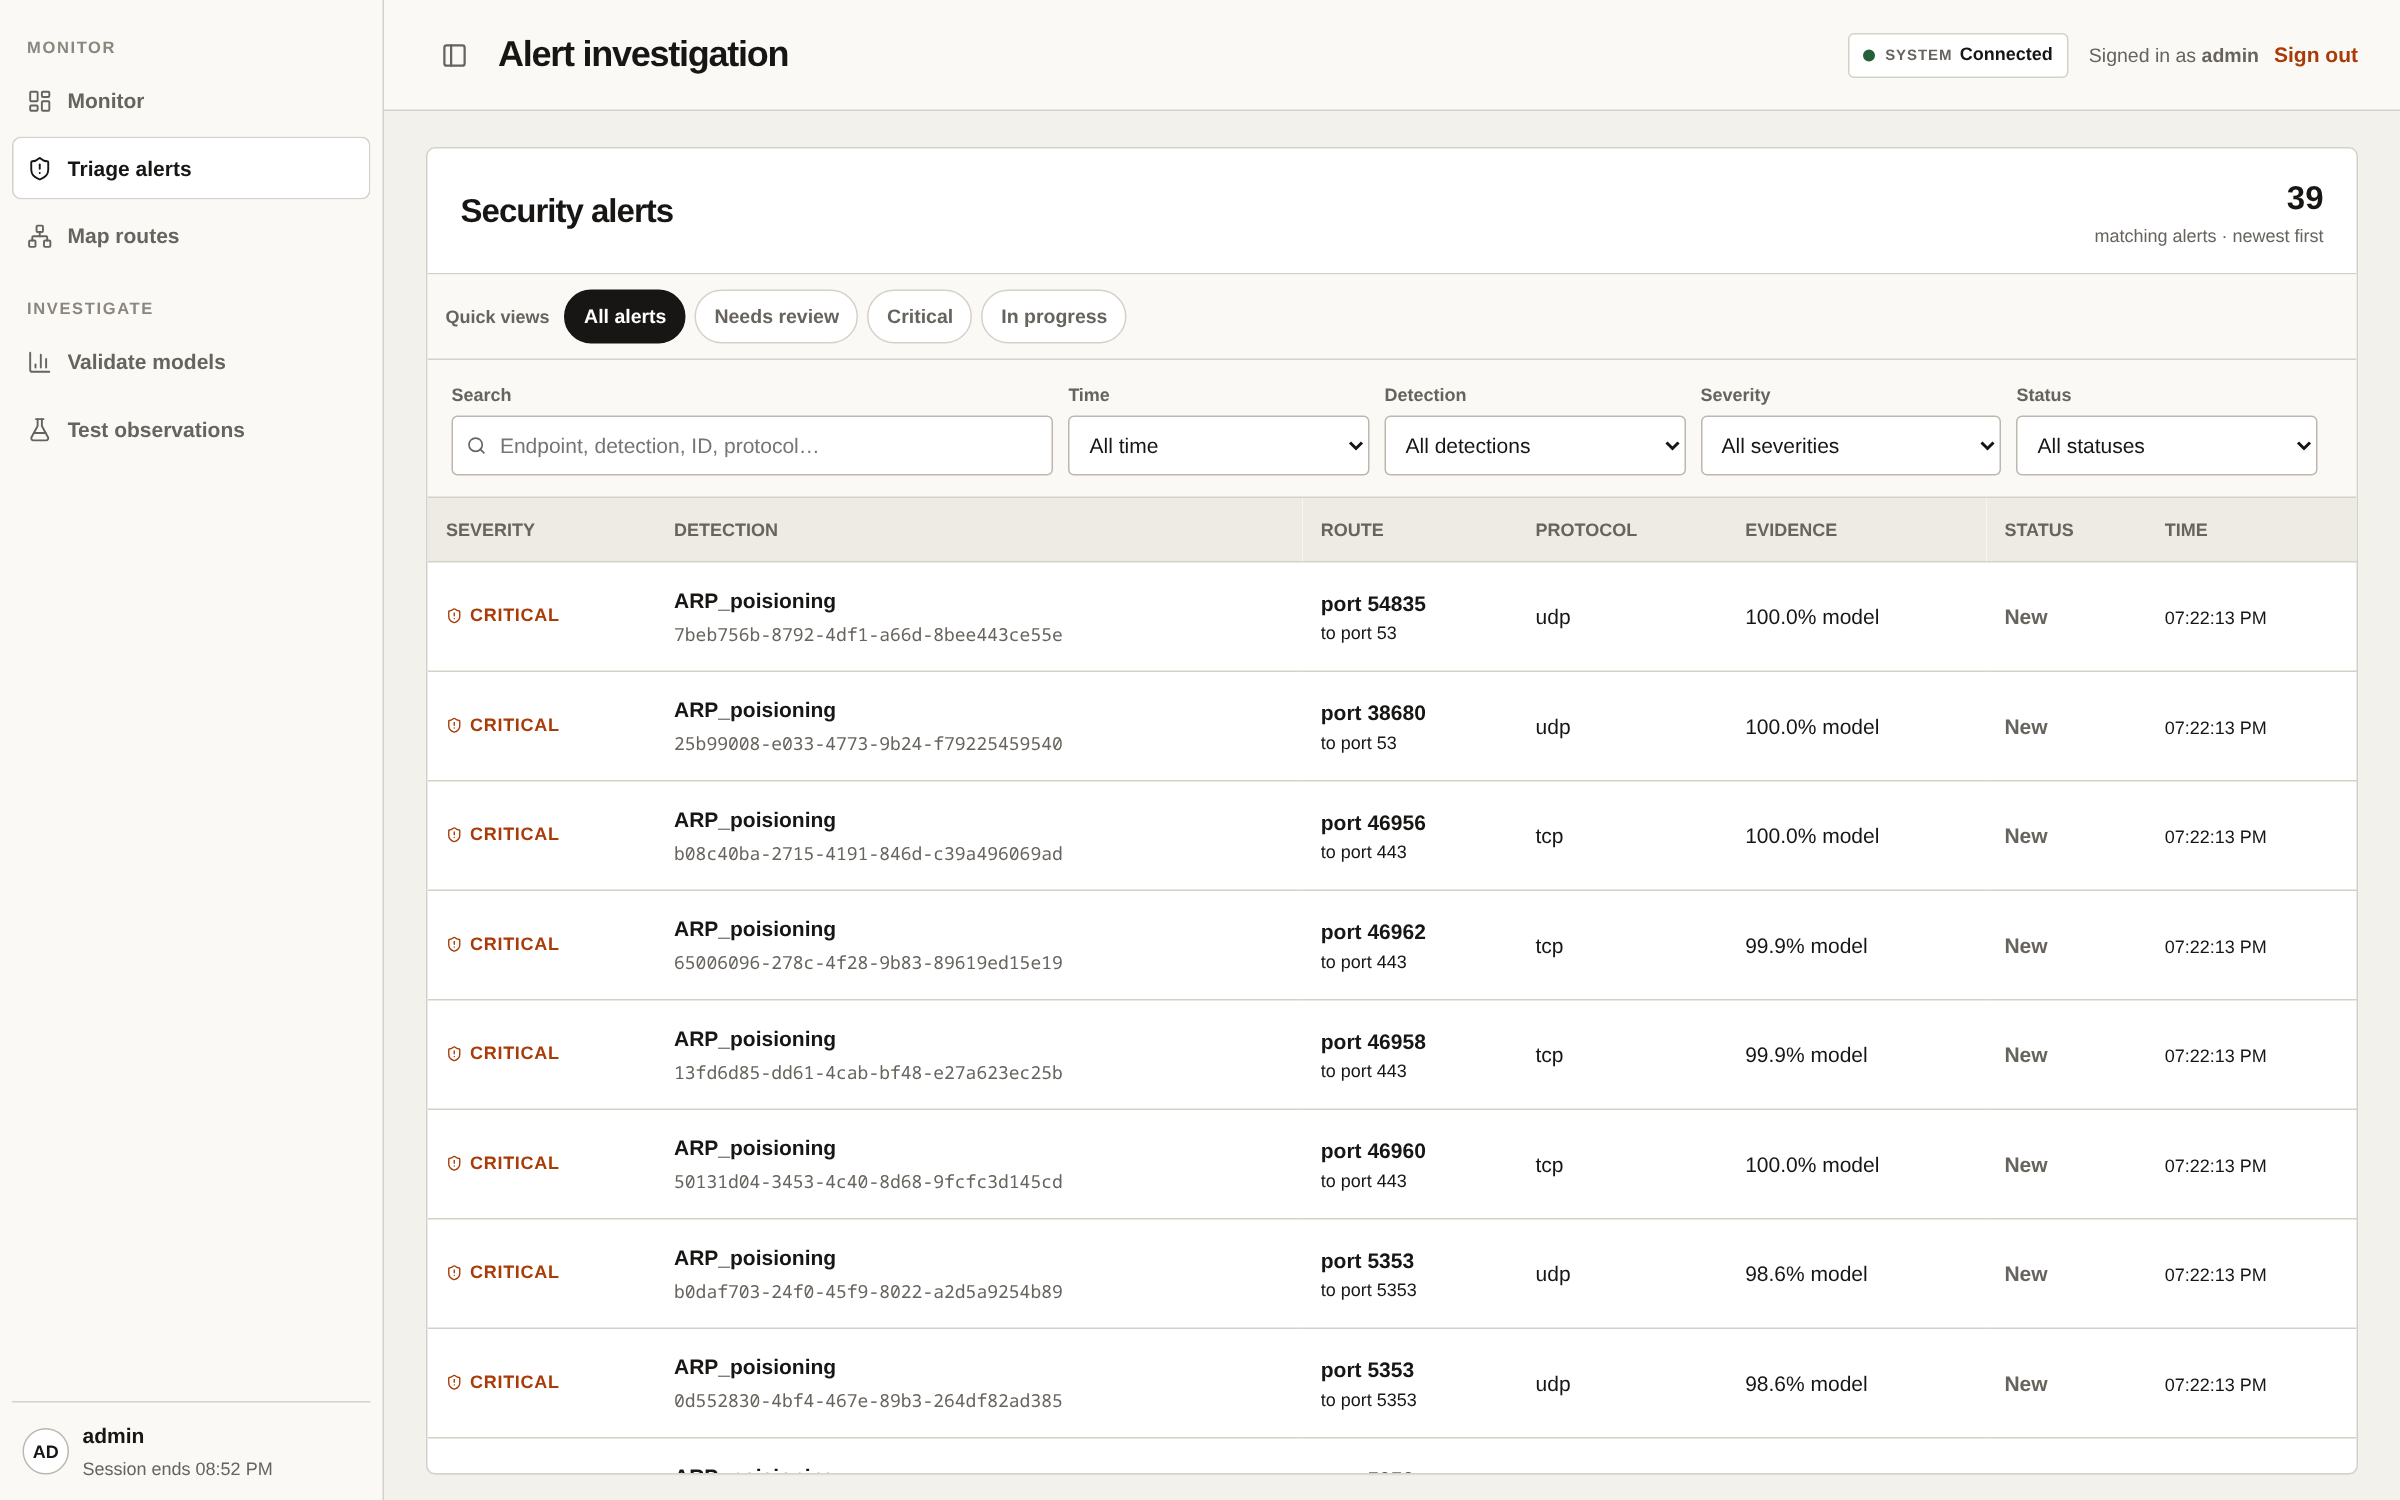
\includegraphics[width=\textwidth,height=0.65\textheight,keepaspectratio]{assets/screenshots/application-alert-investigation.png}
  \caption{Espace d'investigation des alertes}
  \label{fig:implementation-alerts}
\end{figure}

\clearpage
\subsection{Analyse des mod\`eles}

La figure~\ref{fig:implementation-models} expose les artefacts actifs et leur
protocole d'\'evaluation. Les mesures sont pr\'esent\'ees avec leur partage, leurs
graines et leurs limites pour ne pas transformer un score interne au jeu de
donn\'ees en promesse de d\'eploiement.

\begin{figure}[htbp]
  \centering
  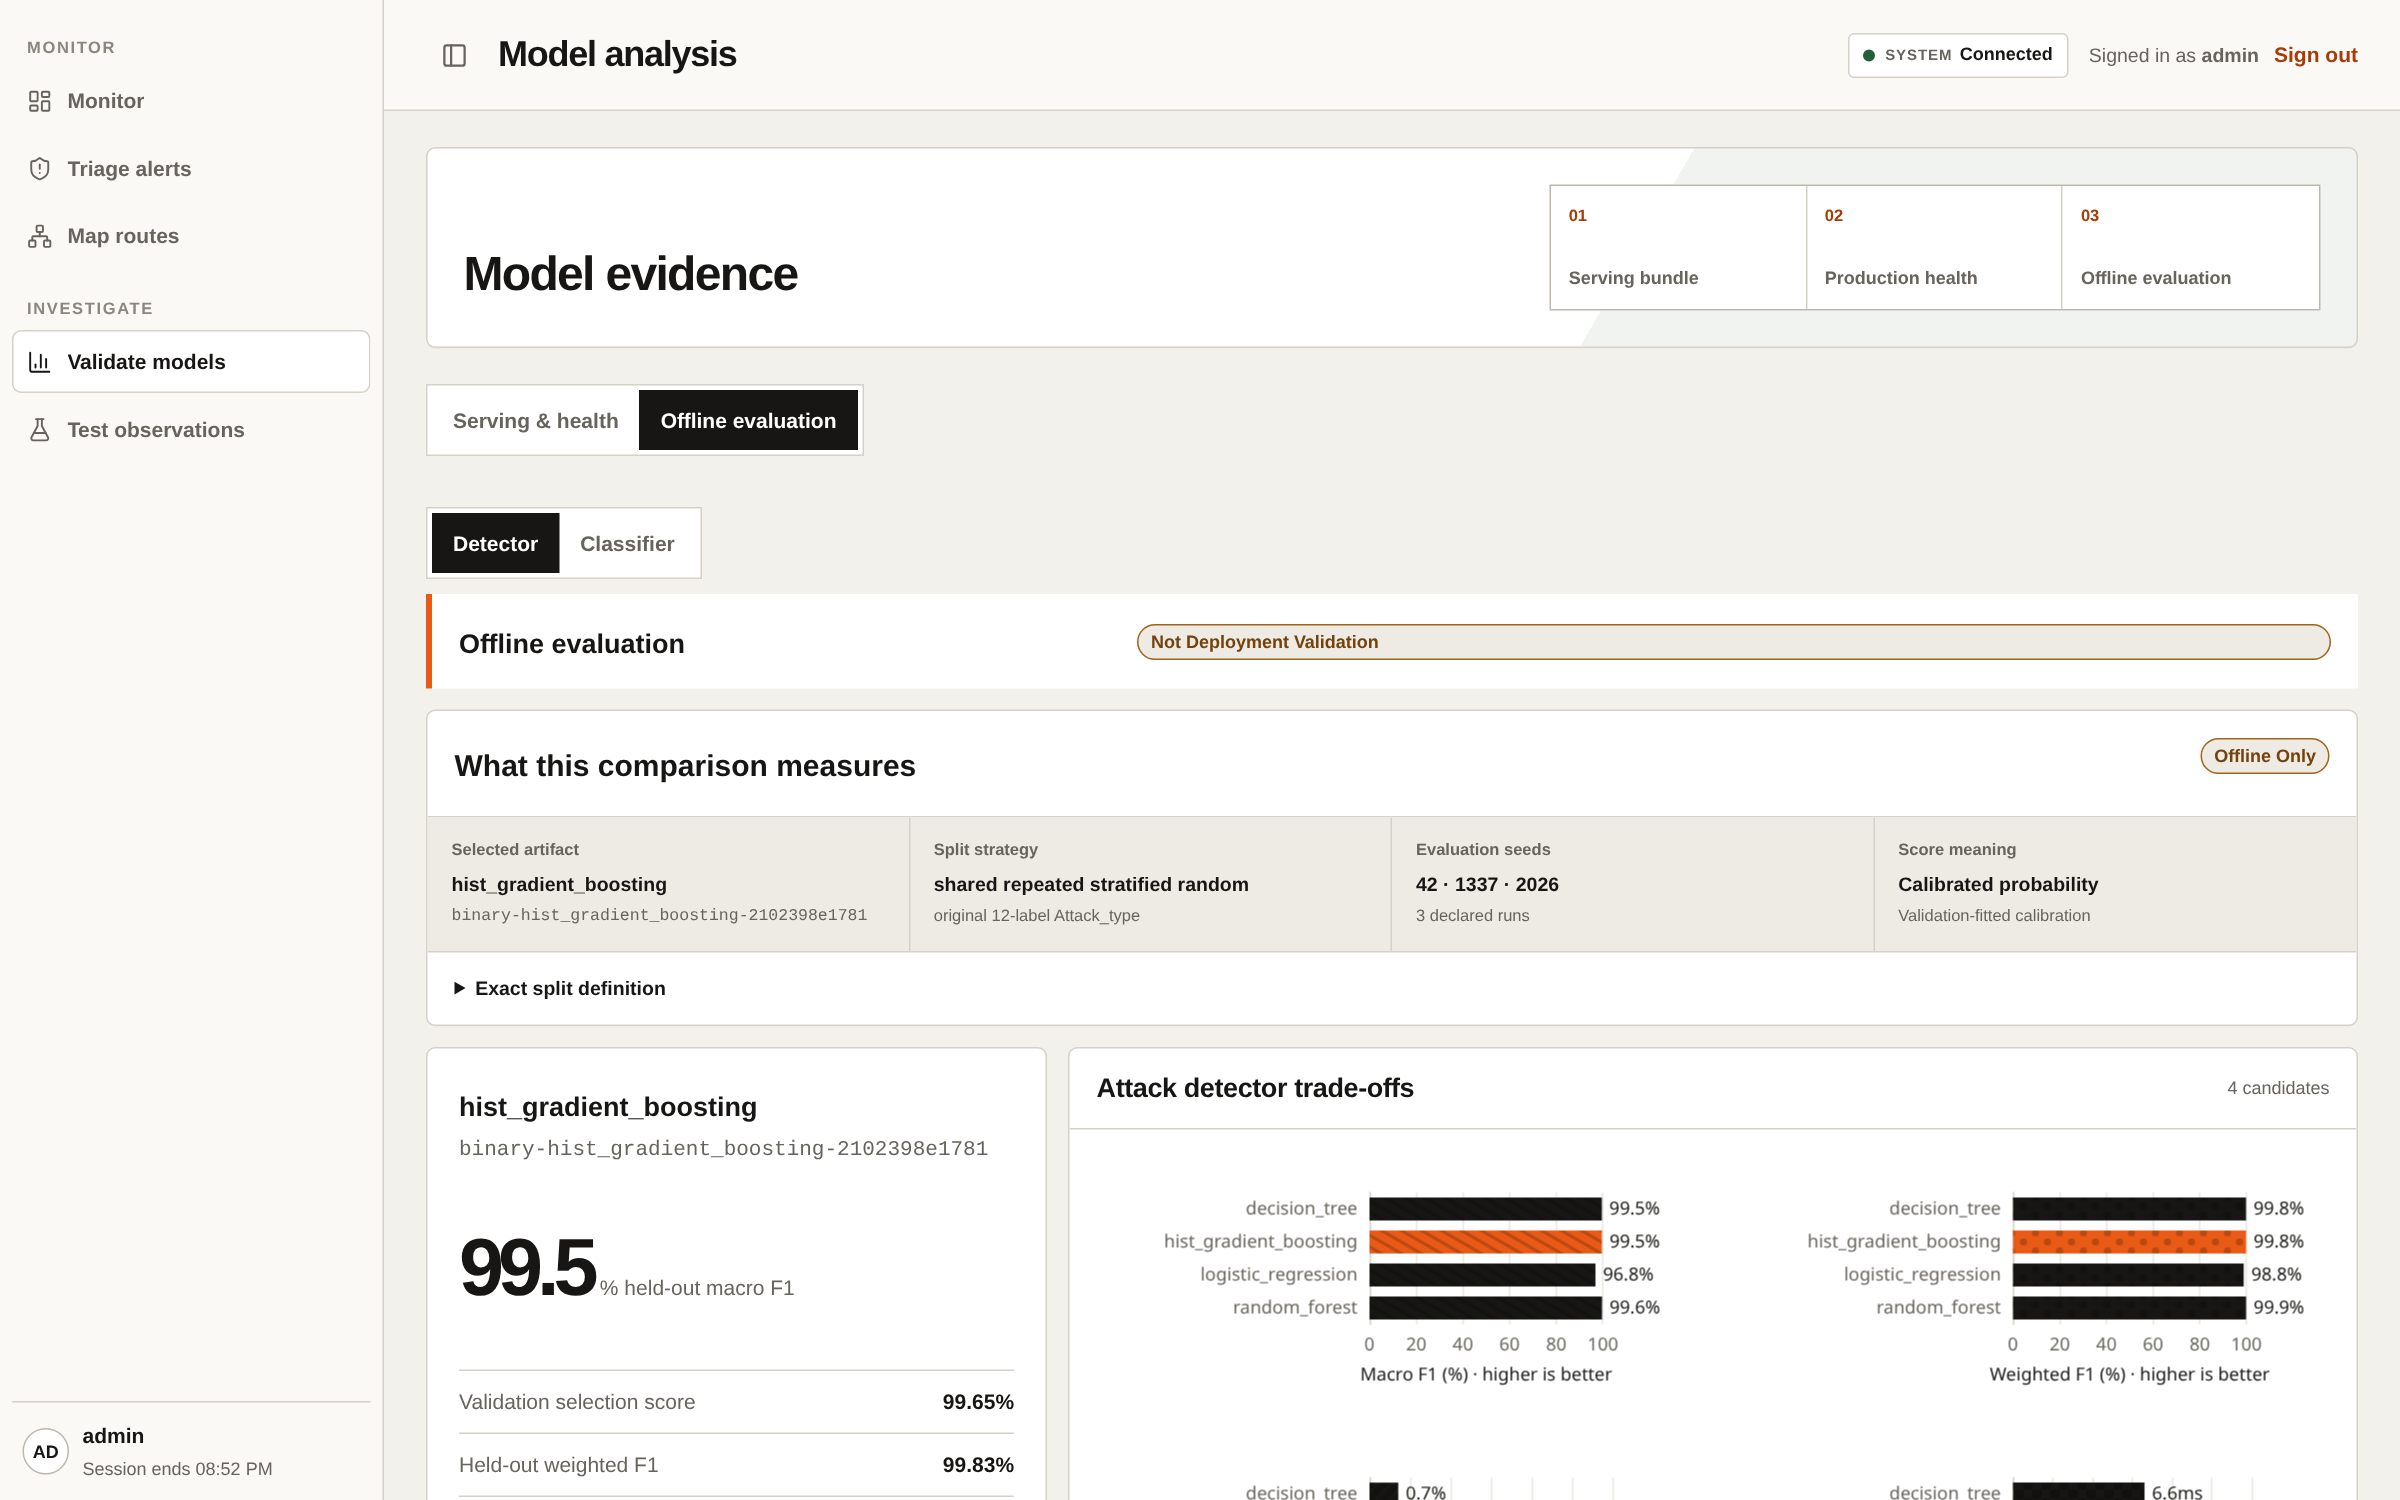
\includegraphics[width=\textwidth,height=0.65\textheight,keepaspectratio]{assets/screenshots/application-model-analysis.png}
  \caption{Espace d'analyse et de tra\c{c}abilit\'e des mod\`eles}
  \label{fig:implementation-models}
\end{figure}

\clearpage
\subsection{Laboratoire d'observations}

La figure~\ref{fig:implementation-lab} permet de contr\^oler une observation ou
un petit lot avant soumission. La validation locale fournit un retour pr\'ecis,
mais l'API authentifi\'ee reste l'autorit\'e finale pour l'acceptation.

\begin{figure}[htbp]
  \centering
  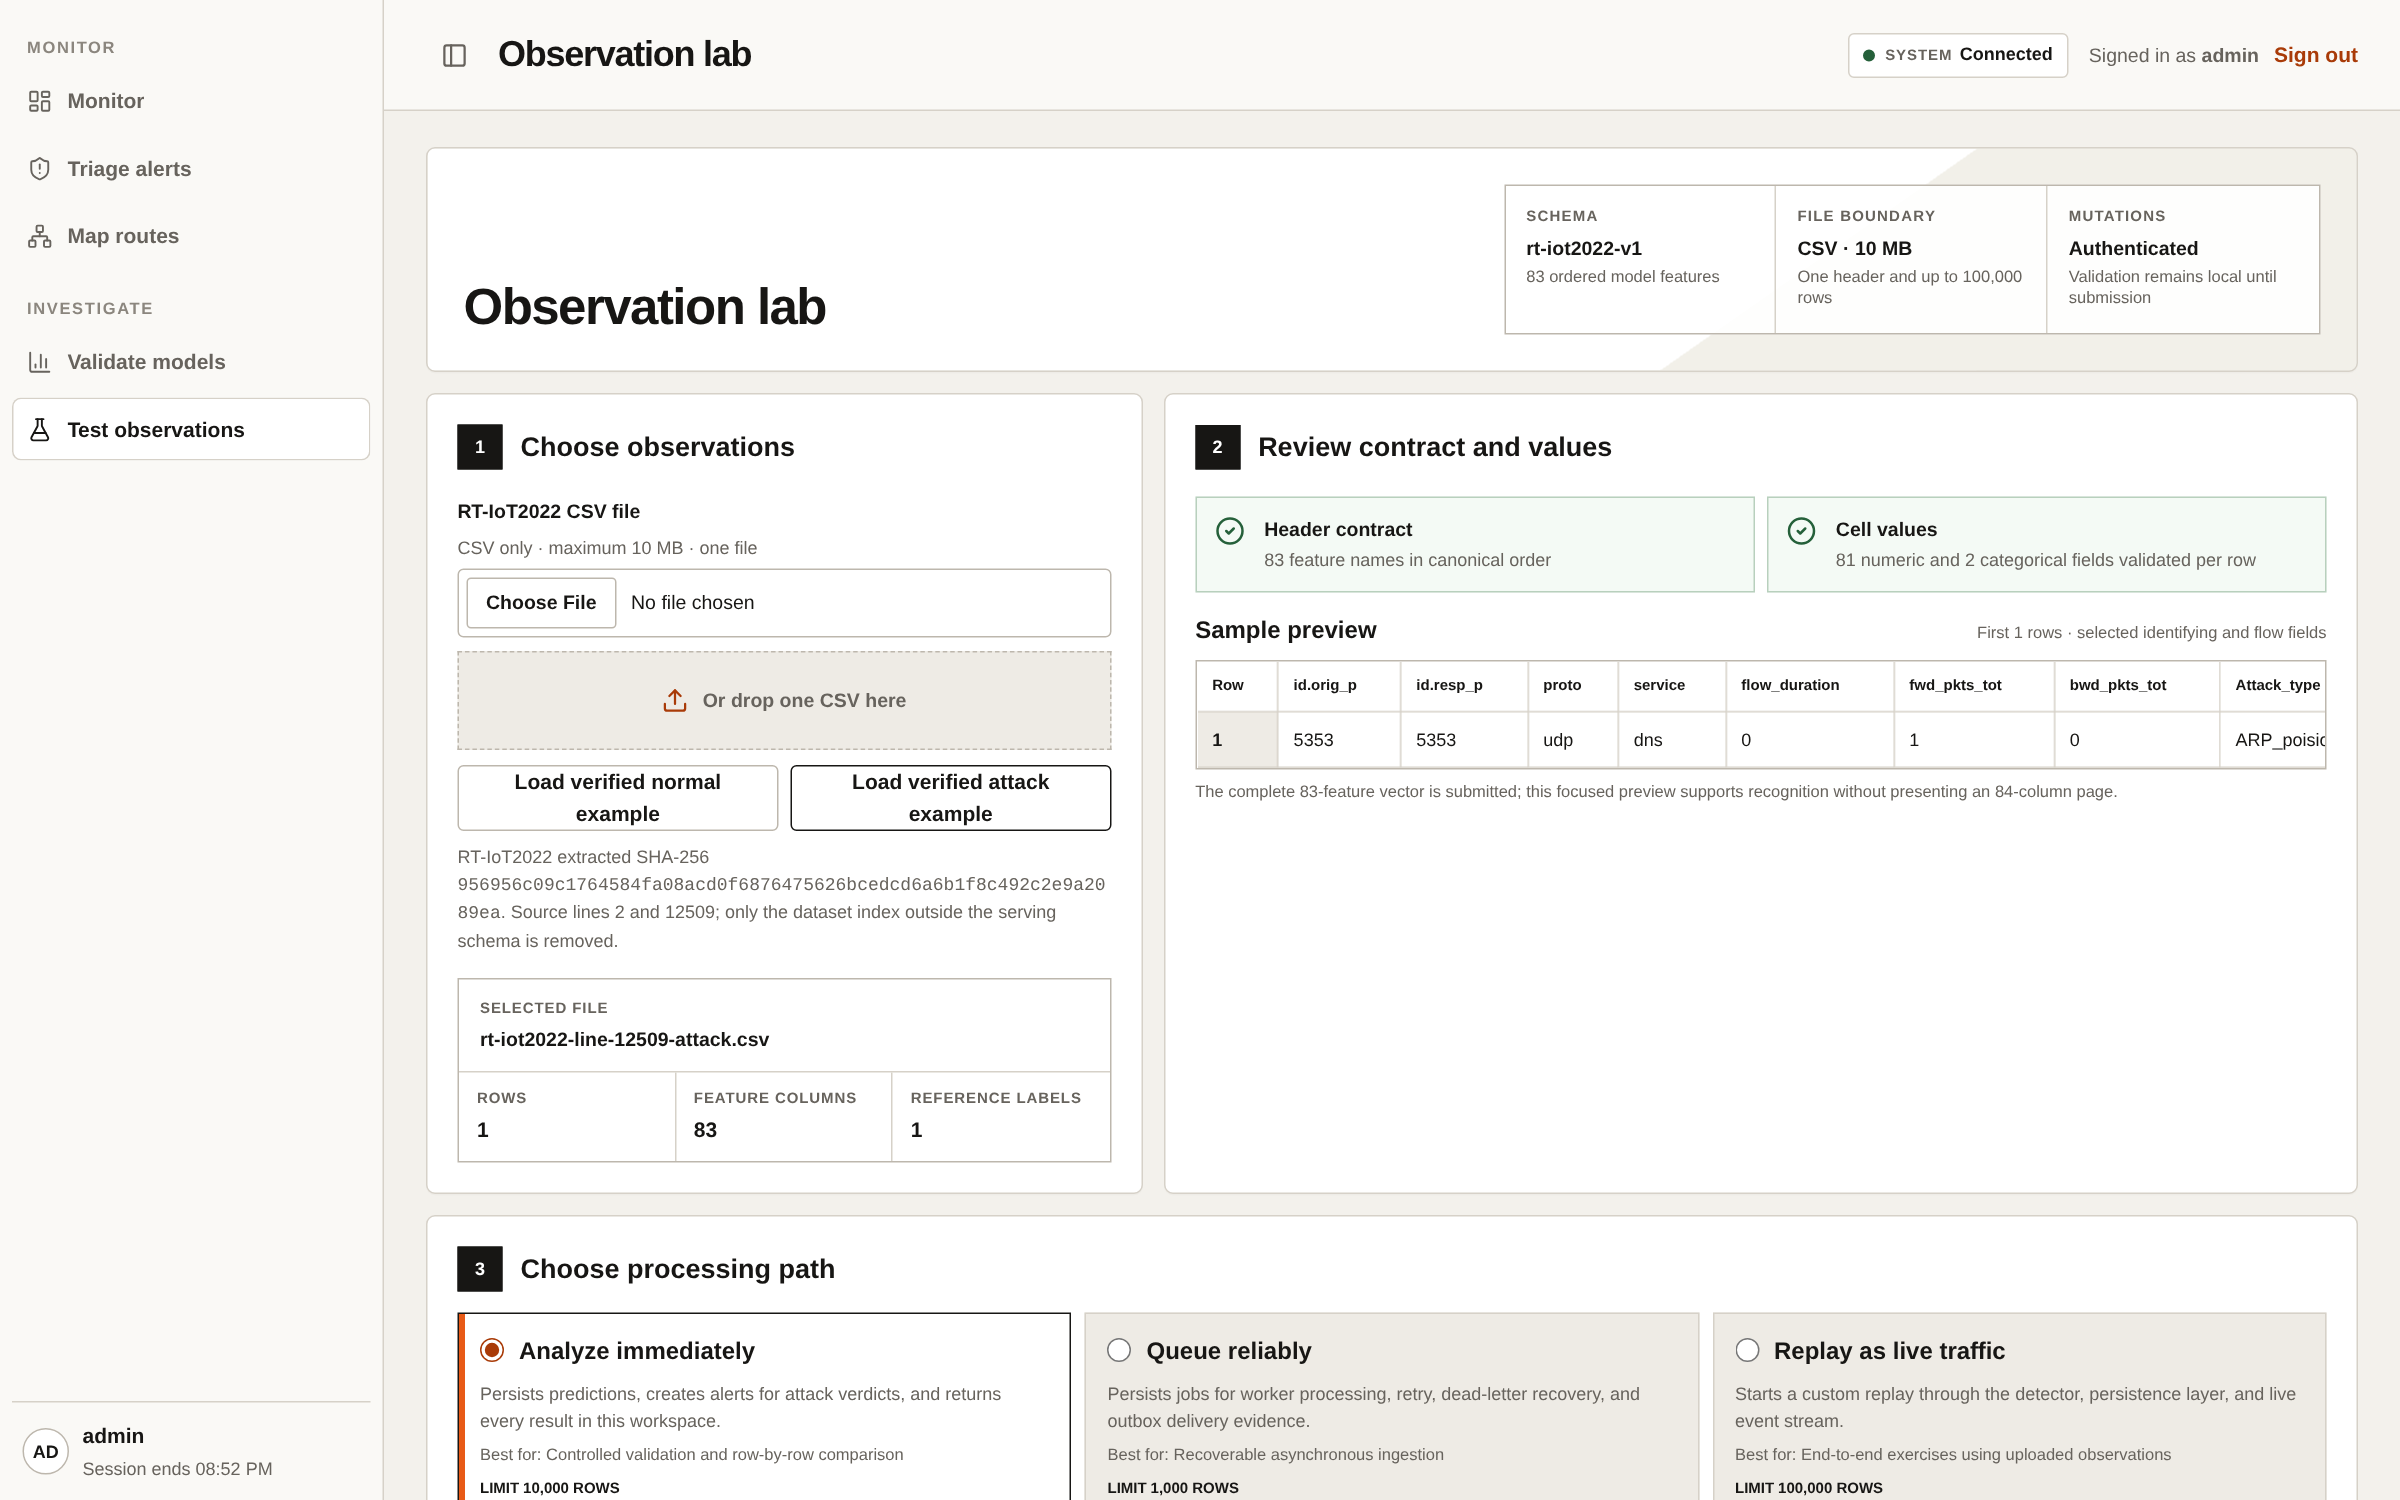
\includegraphics[width=\textwidth,height=0.65\textheight,keepaspectratio]{assets/screenshots/application-observation-lab.png}
  \caption{Laboratoire de validation et de soumission d'observations}
  \label{fig:implementation-lab}
\end{figure}

\section{Validation technique}

La validation automatis\'ee couvre plusieurs niveaux. Les tests Python
contr\^olent pr\'eparation, sch\'emas, promotion, registre, API, persistance,
ingestion, rejeu, sant\'e des mod\`eles et Suricata. Les tests Vitest couvrent les
adaptateurs et composants React. Les sc\'enarios Playwright exercent le parcours
de bout en bout avec les services et les artefacts r\'eels. Les commandes
\texttt{make test}, \texttt{make lint}, \texttt{make build} et
\texttt{make project-preflight} constituent les portes de validation d\'eclar\'ees
par le d\'ep\^ot.

Storybook complète cette validation par des interactions sur les composants
isolés. Des contrôles comparent également les chiffres du support de soutenance
au rapport d'évaluation promu. La répétition complète du 7 septembre 2026 a
validé les dix parcours navigateur, le déploiement Docker temporaire et les
trois scénarios de signature Suricata. Le carnet exécuté et son export HTML
conservent les résultats de cette répétition ; ils attestent du fonctionnement
mesuré, sans démontrer une efficacité sur un réseau externe.

\section{Conclusion}

La r\'ealisation conserve une s\'eparation nette entre apprentissage, service,
persistance et interface. Les m\'ecanismes de validation et de tra\c{c}abilit\'e
rendent la d\'emonstration reproductible, sans supprimer les limites
scientifiques et op\'erationnelles rappel\'ees dans la conclusion g\'en\'erale.
